\documentclass[journal,10pt]{IEEEtran}
\usepackage[T1]{fontenc}
\usepackage[utf8]{inputenc}
\usepackage{newtxtext,newtxmath}
\usepackage{amsmath,mathtools}
\usepackage{booktabs,tabularx,longtable,array,multirow}
\usepackage{graphicx,xcolor,siunitx,microtype,enumitem}
\usepackage{algorithm,algpseudocode}
\usepackage[hidelinks]{hyperref}
\usepackage{url}
\sisetup{group-separator={,},group-minimum-digits=4}
\setlength{\emergencystretch}{1.5em}
\definecolor{peach}{HTML}{FAD6C9}
\definecolor{sage}{HTML}{B0C6A8}
\definecolor{ivory}{HTML}{FAF5E8}
\definecolor{blue}{HTML}{92B3CD}
\definecolor{rose}{HTML}{D99DA3}
\definecolor{mint}{HTML}{D0E3DB}
\definecolor{slate}{HTML}{A6B3C0}
\definecolor{stone}{HTML}{E8E2DB}
\newcommand{\AND}{\mathtt{AND2}}
\newcommand{\OR}{\mathtt{OR2}}
\newcommand{\NOT}{\mathtt{NOT}}
\newcommand{\area}{\operatorname{Area}}
\newcommand{\delay}{\operatorname{Delay}}
\newcommand{\synth}{T_{\mathrm{synth}}}
\newcommand{\cmark}{\ensuremath{\checkmark}}
\newtheorem{proposition}{Proposition}
\newtheorem{lemma}{Lemma}
\title{Truth Table to Circuit: Resource-Aware Synthesis with Shared-DAG Mapping and Bounded Boolean Resynthesis}
\author{Jincan Li and Zeyun Du\\UFUG2106 Discrete Mathematics, HKUST(GZ)}
\markboth{UFUG2106 Final Project Technical Report}{Truth Table to Circuit}
% Generated by integration/verify_evidence.py --write.
\newcommand{\IntegrationRows}{%
1 & Z1 & 50/50 & 1,127,450 & 37.15 \\%
1 & J51 & 50/50 & 1,037,549 & 8.66 \\%
1 & R10.0 & 50/50 & 1,019,547 & 14.74 \\%
1 & Integrated & 50/50 & 872,813 & 32.35 \\%
2 & Z1 & 50/50 & 1,127,196 & 36.95 \\%
2 & J51 & 50/50 & 1,037,549 & 9.42 \\%
2 & R10.0 & 50/50 & 1,019,547 & 15.05 \\%
2 & Integrated & 50/50 & 872,919 & 32.24 \\%
}

\begin{document}
\maketitle
\begin{abstract}
This project converts a complete multi-output truth table into an equivalent AND2/OR2/NOT circuit under gate-specific area and delay costs and per-case computational limits. The independent R10.0 research solver maps exact representations to a shared gate DAG and tests bounded four-leaf rewrites against the whole circuit. The team integration adapts this cut mapper and the Round 5.1 synthesis modules. It also searches variable orders, recovers shared outputs, and repairs late paths. In the pinned release's three public repeats, all 150 circuits passed evaluation, met their delay targets, and passed full truth-table replay. Weighted area ranged from 876,694 to 884,234 per 50-case repeat. A separate matched evaluation compares the integration with submitted Stage 1, the independent Stage 1 freeze, and R10.0. Historical controlled experiments characterize individual passes on their own incumbents.
\end{abstract}
\begin{IEEEkeywords}
Boolean synthesis, truth table, reduced ordered binary decision diagram, DAG rewriting, timing recovery, resource-aware search.
\end{IEEEkeywords}

\section{The Task and the Engineering Question}
\IEEEPARstart{A}{ complete} truth table uniquely specifies a Boolean function, but not its cheapest legal realization. In this project, each input instance gives a vector-valued function
\begin{equation}
F=(f_0,\ldots,f_{m-1}):\{0,1\}^{n}\longrightarrow\{0,1\}^{m},\qquad 1\le n\le20,
\label{eq:function}
\end{equation}
three positive gate-area and gate-delay pairs, a target circuit delay, and optional program runtime and RAM limits \cite{course2026}. A single-threaded program must emit a topologically numbered AND2/OR2/NOT netlist that agrees with \emph{every} row of the table. Logical equivalence alone is insufficient: a correct but deep mapping can lose points, an apparently cheap gate rewriting may delete no actual shared hardware, and a better circuit discovered too late can fail the runtime requirement.

The design question is how to discover a low-area \emph{shared physical network} while preserving target-feasible paths and leaving enough wall-clock time to produce an output. The independent research solver builds a valid incumbent and evaluates bounded changes on the completed DAG. We distinguish the submitted Stage 1 solver (\emph{Z1}), the independent Stage 1 research freeze (\emph{J51}), the independent Stage 2 research freeze (\emph{R10} or \emph{R10.0}), and the final team integration (\emph{Integrated Final}) \cite{stage2integration}. The unified trial log preserves the iterations \cite{stage1research,stage2trial}. The technical derivations and historical figures describe the independent research line. Section~\ref{sec:integration} records the team release and its matched evaluation.

\subsection{The physical and computational objective}
Let \(G=(V,E,O)\) denote the emitted gate DAG with ordered output references \(O\). The project charges \emph{each listed gate once}:
\begin{equation}
A(G)=\sum_{t\in\{\AND,\OR,\NOT\}} a_t N_t(G),
\label{eq:area}
\end{equation}
where inputs, wires, and constant zero cost nothing. In our generator, unused gates are removed before final output, so the sum may equivalently be taken over output-reachable live gates. The latter equivalence must not be assumed for arbitrary unpruned output files. For each source, \(T=0\); for each gate \(v\),
\begin{equation}
T(v)=d_{\operatorname{op}(v)}+\max_{u\in\operatorname{fanin}(v)} T(u),\quad D(G)=\max_{o\in O}T(o).
\label{eq:arrival}
\end{equation}
A unary NOT has one fanin. \(D(G)\) is the propagation delay of the \emph{circuit}; \(\synth\) is the wall-clock runtime of the \emph{program}. Their magnitudes and meanings are unrelated. The grader distinguishes valid PASS from meeting the preferred target \(\Delta\): a target miss penalizes scoring but does not alone make an otherwise valid solution FAIL. Positive execution or memory limits, by contrast, constrain validity \cite{course2026}. We therefore treat a candidate satisfying \(D(G)\le\Delta\) as preferable, without claiming the unpublished numerical scoring rule is known.

The final task has three intertwined decisions: what equivalent Boolean representation to examine, how to map and share its operations in a costed circuit, and how much computational work may be spent searching. These are separate mathematical objects: a truth function \(F\), an abstract functional representation such as a BDD, a physical gate DAG \(G\), and a resource-consuming search program \(\mathcal S\). Most of the project's difficult design decisions arise when an optimization valid at one level does not transfer automatically to the next.

\section{Two Stage 1 Starting Points and the Need for Improvement}
\label{sec:stageone}
\subsection{Actually submitted Stage 1 method (Z1)}
The actual Stage 1 submission (Z1) was already a nontrivial synthesis system \cite{stage1submitted}. It constructs complemented reduced BDDs under several variable orders, maps their decisions into the permitted gate library, explores mapping weights, balances selected gate cones, and retains a completed network using a delay-excess/area/delay ranking. Structural hashing and dead-gate removal account for shared expressions; a finite search allowance limits later candidate trials. Thus the comparison with R10 begins from an optimized Stage 1 circuit, not from a sum-of-minterms straw man. The source-level distinctions, including Z1's sampled influence estimates, are given below.

Z1's physical search chiefly operates through BDD representation and local gate-mapping choices. The independent R10.0 implementation adds a four-leaf cut search over the \emph{already mapped} DAG, an exact streaming affine/literal shortcut for short large-input cases, conservative admission under a positive RAM limit, and two-tier SOP root allocation. The historical whole-solver comparison evaluates these mechanisms together.

\subsection{Independent Stage 1 investigation (J51)}
The independent J51 research line is equally important as a source of the final method's technical ideas, although it was \emph{not} the Stage 1 submitted program \cite{stage1research}. Its early experiments separated \emph{functional correctness} from \emph{costed mapping}: an exact Shannon/ROBDD construction passed all 25 released Stage 1 cases but met only 12 delay targets (area 1,103,455), whereas diversified representations met all 25 targets (area 790,243). Incorporating complemented references and global timing recovery subsequently lowered area to 533,705. The lesson was that representation quality alone cannot determine the cost or critical path of the mapped circuit.

The later J51 work asked a different question: can the same candidate quality be obtained with less synthesis computation? Caching and typed in-memory DAG transformations preserved the observed area 529,014 while reducing paired median runtime. An exploratory four-leaf rewrite branch then found further valid area reductions, but its time penalty prevented promotion to the Stage 1 default. These positive and negative results motivated the Stage 2 combination of \emph{physical-DAG rewriting} with explicit search controls. The complete round-by-round experiments remain in the trial log; the significance here is the chain of technical constraints they exposed.

\begin{table*}[!t]
\centering\caption{Method-improvement map: code-supported distinctions between the submitted Stage 1 solver (Z1) and the independent Stage 2 research freeze (R10). The third column gives the engineering rationale for each change.}
\label{tab:methodchanges}\footnotesize
\begin{tabularx}{\textwidth}{@{}p{.17\textwidth}XXp{.26\textwidth}@{}}\toprule
Question & Submitted Stage 1 (Z1) & Final Stage 2 (R10) & Motivation / measured constraint\\\midrule
How to find the first circuit? & Complemented BDDs, several orders and mapper weights; balancing of mapped gates. & Cached BDD and cover plans, affine recognition, typed DAG balancing and timing recovery. & Retain exactness while reducing repeated search work and evaluating actual graph cost.\\
What structure can be modified? & Primarily BDD-order and Shannon mapping alternatives; limited graph balancing. & Additional four-leaf truth-signature resynthesis directly on the completed physical DAG. & New algebraic structures need not be visible in a BDD-order change.\\
How are local changes judged? & Candidate-level area/delay ranking after construction. & Local cut filtering plus whole pruned-DAG evaluation; multi-output sharing explicitly retained. & Local gate reductions can leave shared ancestors live or alter critical paths.\\
Which candidates get CPU time? & Deterministic order/mapping trials under a fixed search deadline. & Priority-ranked cut roots, separate root quotas, branch time shares, optional strictly improving repeat pass. & Search opportunities, not only nominal time, determined useful R8.6 gains.\\
What happens with tight resource caps? & Keeps the best completed mapping; no specialized affine streaming or comparable RAM admission. & Exact high-\(n\) stream recognition when admitted and conservative positive-RAM fallback. & Stage 2/016 and controlled constrained tests made successful completion a design objective.\\\bottomrule
\end{tabularx}
\end{table*}


\subsection{A source-level comparison, not a one-feature attribution}
The submitted Z1 implementation forms a sequence of at most 32 BDD-order trials, with deterministic first orders, a seeded permutation search, and four mapper weights for later trials. Its influence order is estimated from at most 4,096 sampled truth-table rows. The first complete circuit is constructed before subsequent deadline checks can terminate the search, and the best mapped candidate may be balanced before being returned. This is a substantial, valid Stage 1 synthesis algorithm, not a naive sum-of-products baseline. In contrast, the final R10 implementation computes its influence counts over the full stored truth table, reuses compatible BDD and implicant information across candidates, and performs balancing and area recovery on a typed gate graph. It also exposes completed physical-gate cuts to a \emph{second}, distinct search space. Thus ``more candidate orders'' and ``more cut roots'' are not equivalent notions: the first changes the global functional decomposition, while the second attempts to replace a local portion of a selected mapped implementation.

Table~\ref{tab:methodchanges} therefore compares \emph{systems}, not isolated features. The Z1--R10 pairing asks how the complete solutions perform under the same inputs and execution environment. The much narrower R9.0--R10.0 pairing later tests the marginal value of the guarded SOP postpass. Keeping these questions separate is necessary to explain both the project's overall improvement and the final algorithmic choice.

\subsection{Stage 2's operational trigger}
When the second batch was released, the inherited J51/R7 path could produce a good network yet fail a strict 100-ms case (Stage 2 case 016). R7.1's guarded policy restored pass status but altered some other circuits. R7.2 retained a bounded shortlist to recover quality without reopening expensive late searches \cite{stage2trial}. This episode introduced a principle that remains in R10: \emph{a structurally attractive optimization has no value if the required output is not produced within the evaluator's resource envelope}. In the matched record, Stage 2/016 has \(n=9\) and a declared 100-ms limit. It therefore cannot enter the \(n\ge18\) streaming shortcut or either \(B\ge1000\)-ms cut-search stage. Its later PASS is evidence for the guarded \emph{early} synthesis schedule, not for any gain caused by the final repeat-SOP pass. Once the pass problem was contained, the research shifted toward finding extra equivalent realizations of the completed graph, rather than simply increasing the original BDD-order portfolio.


\subsection{The four design decisions underlying the final method}
Four decisions connect the earlier evidence to the final design. \emph{Representation diversity} supplies several exact starting networks because the smallest abstract BDD need not yield the cheapest gate mapping. \emph{Shared-DAG evaluation} scores the gates that remain physically live across all outputs rather than counting locally removed expressions. \emph{Bounded truth-signature rewriting} searches structural alternatives that the initial representation did not reveal. Finally, \emph{resource-aware allocation} prioritizes and limits this additional work so that circuit improvement does not jeopardize producing a valid netlist. The following sections explain how these decisions fit into one executable synthesis procedure; the evaluation then tests the overall system and isolates selected decisions with controlled contrasts.

\section{The Final Synthesis Architecture}
\label{sec:framework}
Figure~\ref{fig:pipeline} summarizes the ordinary-budget default path; specialized resource-triggered early exits are noted separately. The historical Round names embedded in source files do \emph{not} imply that every archived R8/R9 strategy runs in sequence. With no research environment overrides, the installed postprocessor is R8.6 \texttt{extra\_sop} followed, when admitted, by the R10.0 \texttt{repeat\_sop} pass. Earlier R8.1--R8.5 and R9.1 library modes remain experimental alternatives, not simultaneous stages of normal execution.

\begin{figure*}[!t]
\centering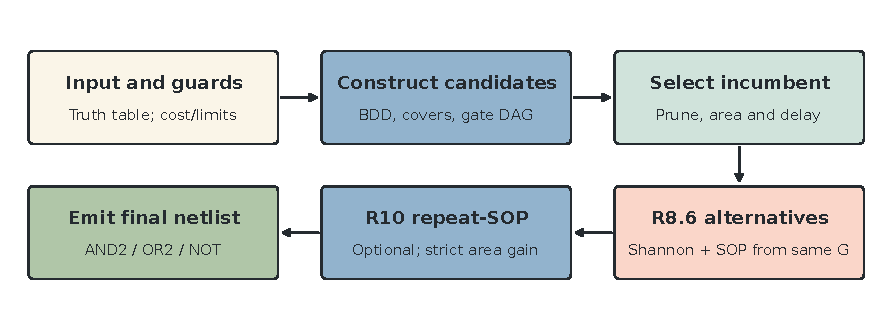
\includegraphics[width=.91\textwidth]{figures/solver_execution_architecture.pdf}
\caption{Source-aligned execution structure of the frozen R10.0 solver. Standard representation candidates are mapped to a shared gate DAG and ranked as full networks. R8.6 tests two cut-search alternatives from the \emph{same} incumbent; R10.0 then tests one additional SOP pass on the \emph{selected} incumbent. Resource-triggered specialized paths are conditional; the diagram is not a guarantee that all optional searches execute.}
\label{fig:pipeline}
\end{figure*}

\noindent\textbf{Executable overview.} Algorithm~\ref{alg:core} states the complete default synthesis controller before the individual mechanisms are derived. It distinguishes the initial, potentially timing-infeasible portfolio from the later optional searches, which require a target-feasible incumbent. The two R8.6 alternatives start from the same graph; the last SOP pass starts from their selected result. Algorithm~\ref{alg:cutrewrite}, introduced after the cut mathematics, specifies the shared local-search subroutine. The displayed controller omits research-only environment overrides and does not imply that every optional pass is activated for every case.\par

\begin{algorithm}[!t]
\caption{R10.0 complete synthesis controller (default policy)}
\label{alg:core}
\begin{algorithmic}[1]
\Require Complete table \(F\), costs \(a,d\), target \(\Delta\), limits \(B,M\)
\Ensure Topological legal-gate netlist or explicit failure
\State Scan table and case parameters; probe exact short-budget families
\If{an admissible exact streaming circuit is on target}
 \State \Return its serialized netlist
\EndIf
\If{positive RAM limit rejects eager construction}
 \State Try compact exact constructor; \Return output or failure
\EndIf
\State Generate BDD/cover mapping candidates within search guards
\State Rebalance, recover area, prune, and rank completed gate DAGs
\State \(G\gets\) best available valid incumbent
\If{R8.6 resource and feasibility admission succeeds}
 \State \(G_S\gets\mathrm{CutRewrite}(G,\mathrm{Shannon},Q)\)
 \State \(G_P\gets\mathrm{CutRewrite}(G,\mathrm{SOP},Q+300)\)
 \State \(G\gets\) best full-network eligible candidate among \(G,G_S,G_P\)
\EndIf
\If{R10 last-pass admission \eqref{eq:lastbudget} succeeds}
 \State \(H\gets\mathrm{CutRewrite}(G,\mathrm{SOP},160)\)
 \If{\(H\) valid, \(D(H)\le\Delta\), and \(A(H)<A(G)\)}
  \State \(G\gets H\)
 \EndIf
\EndIf
\State \Return pruned, topologically serialized \(G\)
\end{algorithmic}
\end{algorithm}

\subsection{Input processing and exact structure detection}
The executable follows the required interface \texttt{synth INPUT OUTPUT}. It first scans the \(2^n\) truth groups and case costs; at high dimension a lightweight streaming probe records whether every output has a simple or affine signature. On the ordinary path, a shared function-cache layer rereads and stores the complete table. This repeated read is real implementation overhead but permits the fast probe to avoid heavier materialization when successful.

For \(n\ge18\) with a \emph{positive} declared time limit \(B\le250\) ms, a recognized all-constant/literal or all-affine output family may be emitted immediately, provided the constructed legal circuit is on target. For affine outputs,
\begin{equation}
 f_j(x)=c_j\oplus\bigoplus_{i\in S_j}x_i,
\label{eq:affine}
\end{equation}
exact recognition uses the complete input table, not sampled extrapolation. XORs are lowered to legal gates using, for example, \(u\oplus v=(u\lor v)\land\neg(u\land v)\), then balanced to control arrivals. Failure to recognize a supported family returns control to general synthesis; it does not justify a heuristic guess about unseen rows.

With a positive RAM cap, a conservative memory estimate may reject eager BDD construction. A compact support-restricted constructor is then tried, and failure may lead to an explicit nonzero exit rather than knowingly running the heavy path. This is a mitigation, \emph{not} a proof of peak-RSS compliance for arbitrary inputs.

\subsection{Functional representation and candidate diversity}
Given a variable \(x_i\), let \(f_0=f|_{x_i=0}\) and \(f_1=f|_{x_i=1}\). Shannon's identity \cite{shannon1949},
\begin{equation}
 f= (\neg x_i\land f_0)\lor(x_i\land f_1),
\label{eq:shannon}
\end{equation}
constructs an exact circuit recursively. Under a fixed order, equal low/high cofactors remove the decision, and identical normalized node triples are interned into a reduced decision DAG \cite{bryant1986}. The code uses complemented references with one inversion bit; this shares Boolean information about \(f\) and \(\neg f\) at representation level without declaring physical NOT gates free. Different variable orders can change decision-DAG size substantially, but neither BDD size nor a compact SOP is by itself the final weighted gate cost. To see the interface between the two representations, the generic Shannon decision has the legal realization
\begin{equation}
 q=\OR\!\left(\AND(\neg x_i,f_0),\AND(x_i,f_1)\right),
 \label{eq:muxlowering}
\end{equation}
which costs at most two AND2s, one OR2 and one NOT \emph{before} constant simplification and sharing of an existing inverter or child expression. Alternative polarity-aware forms can have different prices and arrivals. Consequently, a fewer-node decision DAG does not imply fewer emitted gates; mapping is a separate optimization problem.

For each output and candidate order, the frozen solver considers several physical Shannon and implication-aware realizations, with affine recognition and small-support SOP/POS cover plans when eligible. Its influence-based ordering uses the exact sum of differing cofactors over output bits,
\begin{equation}
 C_i=\sum_{x_{-i}}\sum_{j=0}^{m-1}\mathbf 1\{f_j(x_{-i},0)\ne f_j(x_{-i},1)\},
\label{eq:influence}
\end{equation}
not as a minimum-area theorem but as a way to prioritize potentially decisive variables. Symbolic implicant plans for manageable support are cached independently of physical gate emission. This separation avoids recomputing equivalent Boolean analysis for several mapper policies, but makes no claim that a greedy cover minimizes the eventual shared circuit's cost \cite{brayton1984}.

\subsection{Typed gate-DAG mapping and global recovery}
Each candidate is mapped to a typed internal graph whose nodes have an operator and one or two earlier fanin references. AND/OR input IDs are sorted for commutative structural hashing. Its builder simplifies constants and duplicates, rebalances eligible associative cones, and creates shared gate nodes; a final backward traversal from all outputs removes speculative unreachable gates and topologically renumbers the rest. The graph retains per-node forward arrival times, avoiding repeated text serialization and reparsing during high-frequency transformations.

An associative subgraph can be flattened and rebuilt only when this does not silently remove a still-shared intermediate. In particular, a gate with multiple consumers is a physical signal with a lifetime beyond one parent expression. Required-time recovery calculates the latest admissible arrival \(R(u)\) by initializing \(R(o)=\Delta\) at every output and propagating the minimum backwards along old graph edges:
\begin{equation}
 R(u)\leftarrow\min\big(R(u),R(v)-d_{\operatorname{op}(v)}\big),\quad u\in\operatorname{fanin}(v).
\label{eq:required}
\end{equation}
Shared fanout imposes the tightest downstream constraint. The slack \(S(u)=R(u)-T(u)\) may permit De Morgan and algebraic alternatives that are individually slower but cheaper under heterogeneous gate prices. However, old required times provide a sufficient timing certificate only for a replacement with unchanged external dependencies. The program consequently recomputes the entire candidate's delay, rather than treating a local arrival check as proof for arbitrary global restructuring.

\begin{lemma}[Fixed-boundary timing condition]
Suppose an initially target-feasible acyclic network is modified only by Boolean-equivalent replacements whose exposed roots connect to an otherwise unchanged downstream graph. If every new root arrival is at most the corresponding \emph{old} required time computed using Eq.~\eqref{eq:required}, then the modified network still meets target \(\Delta\).
\end{lemma}
\begin{IEEEproof}
The old backward recurrence guarantees \(R(u)+d(v)\le R(v)\) along every unchanged edge \(u\to v\). The replacement root hypothesis supplies the base case. Topologically, for each unchanged gate \(v\),
\[
 T'(v)=d(v)+\max_{u\in\operatorname{fanin}(v)}T'(u)
 \le d(v)+\max_{u}R(u)\le R(v).
\]
Thus every output arrival is bounded by its old requirement, at most \(\Delta\). The proof relies on the unchanged boundary: arbitrary fanout modifications invalidate this inference without fresh analysis.
\end{IEEEproof}


\paragraph{The cost of graph recovery is not a Boolean gate-count proxy.}
The source's \texttt{area\_recover} considers a complemented physical realization only when its isolated gate prices justify a conservative test. For example, it considers converting a costly OR2 to a complemented AND2 pattern when
\begin{equation}
 a_{\lor}>a_{\land}+3a_{
eg}.
 \label{eq:demorganscreen}
\end{equation}
This is an implementation-level \emph{screening condition}, not a necessary condition for a globally profitable De Morgan rewrite: the three inversions may be partly shared or eliminated, but an apparently removable gate may still be live for another output. The source separately checks the new node's forward arrival against the old required-time bound and then scores the reconstructed graph. Thus even the older Stage 1 machinery already contains a distinction between a sufficient local price condition and the final mapped cost; Stage 2 applies the same principle to a larger space of exact local functions.

The completed candidate portfolio is ranked by an internal delay-violation-first, then area/delay preference. A compact characterization is
\begin{equation}
 \rho(G)=\Big(\max(0,D(G)-\Delta),\;\mathbf1_{D(G)\le\Delta} A(G),\;D(G),\;A(G)\Big),
 \label{eq:rank}
\end{equation}
compared lexicographically among valid completed candidates. This is the program's policy; it is not the unpublished course grading function. Crucially, optional later searches are entered only after a completed incumbent exists, so their failure need not erase already constructed output.

\subsection{What can actually run before cut rewriting}
The ordinary path does not jump directly from a truth table to a four-leaf cut search. The first portfolio has five baseline configurations: several influence-descending mappings that differ in polarity or implicant modes, plus one natural-order realization. Some duplicate implicant settings are omitted once their support-dependent mechanism is inactive. Reverse, rotated and ascending-influence order candidates are only admitted when both input dimension and declared time budget allow them. Each completed candidate is parsed into a typed graph, optionally rebalanced and recovered, and compared by Eq.~\eqref{eq:rank}; the selected incumbent is then eligible for further processing. Under sufficiently generous budget, additional legacy mappings and shallow algebra/phase alternatives can also be compared before the cut stage. They are \emph{not} R8.6 cut branches, and their contributions cannot be inferred from the R9.0--R10.0 ablation.

This ordering has an important implementation consequence: \emph{when} the expensive search is attempted depends on the existence of a complete earlier circuit. A sufficiently small positive runtime allowance can suppress the legacy portfolio and all later cut searches. In contrast, when the first candidate already has area and delay zero, optional work is skipped as no nonnegative gate-cost improvement is possible. These admission checks do not mathematically guarantee an output on every future bounded instance, but they make the completed incumbent the organizing unit of the source's search schedule.

\subsection{A hierarchy of exactness, cost, and search effort}
The final pipeline operates on three different objects whose metrics must not be substituted for each other. The stored truth table specifies the exact vector function $F$; the mapped and pruned gate network $G$ is the physical artifact charged by Eqs.~\eqref{eq:area}--\eqref{eq:arrival}; and the synthesis procedure $\mathcal{S}$ explores alternatives while spending wall-clock time and memory. Consequently, a step may be useful for three different reasons: it may enlarge the set of \emph{exact} circuits that can be constructed, find a cheaper completed network among those circuits, or reduce the cost of exploring the same candidates. Stage 1 established the first and third possibilities through ROBDD construction, diverse mapping and typed-graph caching; Stage 2 specifically extends the second through bounded function-level rewriting under the third's resource constraints.

For clarity, let $G_0$ be the completed incumbent after representation search, mapping, balancing and recovery. The R8.6 controller produces two \emph{alternative} searches from that same network, not two sequential transformations:
\begin{equation}
\mathcal{C}(G_0)=\{G_0,\;H(G_0;Q_H),\;P(G_0;Q_P)\},
\label{eq:parallel_candidates}
\end{equation}
where $H$ denotes the bounded Shannon-oriented cut search and $P$ the bounded SOP-oriented search, subject to their actual eligibility and time guards. A completed candidate is evaluated using the \emph{whole} pruned shared DAG. The controller chooses a valid preferred candidate $G_1$ from available eligible results. If the R10.0 final-pass guard subsequently admits more work, it applies a \emph{new} SOP pass to $G_1$, not to the original $G_0$:
Set $\widehat G=P(G_1;160)$. The return rule is
\begin{equation}
G_{\rm out}=\begin{cases}
\widehat G, & \text{if $\widehat G$ passes the strict admission test},\\
G_1, & \text{otherwise},
\end{cases}
\label{eq:two_level_choice}
\end{equation}
where the admission test checks structural validity, $D(\widehat G)\le\Delta$ and $A(\widehat G)<A(G_1)$, while functional equivalence follows from the constructor's exact transformations under the hypotheses proved below. The acceptance function does \emph{not} rerun an independent exhaustive truth-table equivalence checker for every new candidate.
Equation~\eqref{eq:two_level_choice} describes the \emph{admission rule} after a returned candidate, not a universal bound on the time taken by candidate construction. In particular, one cannot sum the isolated R8.6 root-allocation gain and the R10.0 postpass gain as if both acted on an unchanged graph: the second pass sees the fanout structure and available cuts produced by the first decision. This distinction is the organizing principle of the final method, not a detail about how many development rounds were run.

\section{Core Stage 2 Improvement: Bounded Cut Resynthesis}
\label{sec:cut}
\subsection{Why BDD-order search is not sufficient}
Changing a BDD order changes the decomposition of the whole function. Yet the mapped gate DAG may contain a locally expensive algebraic pattern even if its original BDD representation was compact. The Stage 2 method instead treats a bounded portion of the \emph{existing physical circuit} as a small Boolean function, reconstructs an alternative expression for that function, and measures whether replacing it changes the complete shared circuit favorably. The idea is related to established DAG-aware rewriting \cite{mishchenko2006}, but the implemented cut size, exact local signature, root ranking, and gate prices are specific to this project.

\subsection{A running example: equivalence, sharing, and timing}
Consider
\begin{equation}
 y_1=(a\land b)\lor(\neg a\land c),\qquad y_2=y_1\lor b.
\label{eq:example}
\end{equation}
Using one NOT, two AND2, and two OR2 gates, with areas \((a_{\land},a_{\lor},a_{\neg})=(2,3,1)\) and delays \((d_{\land},d_{\lor},d_{\neg})=(2,2,1)\), the initial shared network has area \(11\), output arrivals \(5\) and \(7\), and global delay \(7\). With target \(8\), the \(y_1\) node is also the predecessor of the final OR2 producing \(y_2\); its required time is \(\min(8,8-2)=6\), not \(8\). Absorption gives \(y_2=b\lor(\neg a\land c)\). Redirecting only the final OR2 to the existing \((\neg a\land c)\) node preserves both outputs, leaves the gate producing \(y_1\) alive as the first output, and changes the \(y_2\) arrival from \(7\) to \(5\) \emph{without changing area}. It also changes the fanout graph and the new required time of \(y_1\) to \(8\). The example isolates three notions often confused in heuristic optimization: Boolean equivalence, actual live-gate reclamation, and critical-path timing.

\subsection{Cut boundaries and functional signatures}
The running example permits an algebraic simplification by inspection. To discover such opportunities systematically, the solver first recovers the Boolean function of a bounded region of the \emph{already mapped} DAG. For a root gate \(r\), a cut \(C_r=\{\ell_0,\ldots,\ell_{k-1}\}\) is an upstream frontier crossing every path from \(r\) toward primary inputs. The implementation restricts \(1\le k\le4\), forming sorted unions of fanin cuts while keeping only a bounded number of representatives per node. Each internal node retains its trivial self-cut, one available cut of each cardinality, and at most nine retained cuts in all. This diversity-preserving cap is a design choice: it prevents an exponential blow-up of cut combinations but can discard a functionally valid frontier that would have mapped better. Cut count therefore limits \emph{search coverage}, not Boolean exactness of any candidate actually tested. It is \emph{not} an exhaustive enumeration of all possible four-leaf cuts. Treat the cut leaves as formal Boolean variables \(z_0,\ldots,z_{k-1}\). The local function can be encoded exactly as
\begin{equation}
 M_{r,C}=\sum_{s=0}^{2^k-1} h_{r,C}(s)\,2^s \;\in\; \{0,\ldots,2^{2^k}-1\}.
\label{eq:cutmask}
\end{equation}
With four leaves this signature uses only 16 bits. The actual routine in \texttt{r84\_cut.hpp} orders the leaf IDs increasingly and uses the \emph{least significant assignment bit} for the first leaf: \(s=\sum_{i=0}^{k-1}2^i z_i\). A recursive evaluation replaces every leaf by its formal truth-mask, AND/OR by bitwise operations and NOT by masking the complement. If a path reaches a primary input without passing a designated leaf, the proposed cut is invalid rather than approximately accepted.

\begin{proposition}[Functional validity of cut replacement]
Let \(C_r\) be a valid cut and \(h_{r,C}\) its induced function on formal cut-leaf values. Replacing the root cone by an acyclic legal-gate expression \(\widetilde h\) with \(\widetilde h(z)=h_{r,C}(z)\) for every \(z\in\{0,1\}^k\), while preserving the graph boundary and all dependent outputs, preserves the full multi-output function.
\end{proposition}
\begin{IEEEproof}
For each original input assignment \(x\), the actual vector of cut-leaf signals \(z(x)\) is one member of \(\{0,1\}^k\). The signature equality holds on \emph{every} such vector, even if the physical leaves are mutually dependent and not all vectors are realizable. Hence \(\widetilde h(z(x))=h_{r,C}(z(x))\). All downstream gates receive the same root value and all other unchanged signals retain their values; induction through the remaining topological graph preserves each output.
\end{IEEEproof}

This proposition proves local functional equivalence under explicit wiring and acyclicity assumptions. It does not, by itself, establish legality of the replacement's indices, reduced area, or a satisfactory timing path.

\paragraph{An explicit cut signature and its physical interpretation.}
The multi-output function in Eq.~\eqref{eq:example} supplies a concrete cut: take the root computing $y_2$ and the formal leaves $(a,b,c)$, with assignment index $s=4a+2b+c$. Its on-set is $\{1,2,3,6,7\}$, hence the exact eight-bit signature is
\begin{equation}
M_{y_2,\{a,b,c\}}=2^1+2^2+2^3+2^6+2^7=206=\texttt{0xCE}.
\label{eq:maskexample}
\end{equation}
This display follows the Stage 1 running example's human-readable convention, where $a$ is the \emph{most} significant bit. Under R10's actual leaf-bit convention, $s=a+2b+4c$ for sorted leaves $(a,b,c)$, and exactly the same function has mask $220=\texttt{0xDC}$: neither value is canonical without specifying leaf order and bit significance. Both the original $y_1\lor b$ cone and the alternative $b\lor(\neg a\land c)$ have this signature under a fixed convention. The equality certifies the functional substitution; the unchanged area and improved delay calculated in the preceding example are \emph{separate} properties of its mapped, shared circuit. Neither one follows solely from the truth mask.

\subsection{Generating replacement expressions}
For each feasible truth signature, the local synthesizer considers: (i) SOP based on prime implicant enumeration with two deterministic greedy uncovered-cover proxies; (ii) complemented SOP or POS-flavored realizations; and (iii) selected Shannon decompositions and leaf-order rotations. Every candidate is lowered to AND2/OR2/NOT through the same typed builder. A greedy implicant cover is correct when its terms stay within the on-set and jointly cover the entire on-set, but this does not minimize weighted physical gate area after structural sharing. A Shannon alternative is exact by Eq.~\eqref{eq:shannon}, but can increase gate count while reducing critical-path depth. These candidates are \emph{semantically complete for the chosen expression}, not exhaustive for all possible circuit implementations.

\paragraph{What is actually enumerated in the frozen cut engine.}
The SOP path enumerates all cube patterns over the \(k\le4\) formal leaves, discards cubes covering a zero minterm, retains prime implicants, and builds a greedy cover under either of two cost proxies. It also synthesizes the complemented truth mask and negates the result, exposing a POS-like alternative without introducing an illegal physical gate. The Shannon path tests up to four rotations of the \(k\)-leaf decision order. These local realizations use an immutable cut truth signature; a builder may intern common AND/OR/NOT gates across speculative expressions. The retained set is intentionally small enough to be searched repeatedly across a large output DAG. It cannot be described as all Boolean functions' minimum-area implementations, nor should the two greedy cover proxies be interpreted as an exhaustive search over all prime-implicant covers.

\subsection{Why local area estimates cannot decide globally}
The example also shows why discovering an equal truth signature is only the first step. To judge whether the substitution is desirable, the solver must account for all outputs and shared gates. Define \(L(G)\) as the union of all gate ancestors of the output references, including output gates. For a pruned graph the area is \(\sum_{v\in L(G)}a(v)\). If gates in the old and new graphs are compared under a \emph{common immutable gate identity} (operator together with recursively identified fanins), unchanged shared nodes have the same cost, and for a rewrite from \(G\) to \(G'\),
\begin{equation}
\begin{split}
 A(G')-A(G)={}&\sum_{v\in L(G')\setminus L(G)} a(v)\\
 &-\sum_{v\in L(G)\setminus L(G')} a(v).
\end{split}
\label{eq:delta}
\end{equation}
Equation~\eqref{eq:delta} requires stable structural node identities: gate IDs from independently serialized networks cannot be subtracted as sets. The practical consequence is visible in the running example. Eliminating a \emph{use} of a shared node does not eliminate its area, whereas replacing a root may release several private ancestors at once. Global improvement must ultimately be measured from each complete output-reachable network.

The cut engine makes this evaluation affordable with an earlier, conservative screen. It estimates \emph{reclaimable private area} by walking the old cone, stopping at cut leaves or multiply used non-root nodes, and capping unusually large walks at 80 nodes. It constructs a candidate against the same frontier and normally requires its estimated local cost to beat that reclaimable area (an equality-enabled research mode is available). The candidate must also meet the old root's required arrival. These conditions prune likely unprofitable rewrites; they do not prove that the predicted gates will disappear. After the full DAG is reconstructed and pruned, the outer policy recomputes its actual area and delay before acceptance.

This two-stage test makes a tradeoff explicit. A false optimistic local estimate cannot force a worse completed incumbent to be accepted, because the full-network test remains authoritative. A false pessimistic estimate, however, can \emph{miss} a globally useful transformation: local estimation is deliberately conservative, and the finite cut and root quotas further limit coverage. These are algorithmic limitations, not implementation errors or Boolean approximations.

\subsection{Timing and final acceptance}
Before materialization, an alternative root is rejected if its estimated arrival exceeds the old \(R(r)\). This is an inexpensive local filter, not a complete global feasibility theorem when dependencies change. The rewritten graph is constructed with the original outside DAG preserved, pruned, and scored. At the outer R8.6 policy, a candidate is eligible when valid and on target and is either strictly smaller in area than the original baseline or has equal area with smaller delay. The final R10 follow-up uses a stricter condition: area must decrease. The algorithm always prefers the completed incumbent to an invalid or unacceptable new candidate.

\subsection{Root priority and deterministic work limits}
When many roots exist, a naive scan spends effort on arbitrary graph positions before reaching promising structures. The implemented priority score for an eligible root \(r\) is
\begin{equation}
\begin{split}
 P(r)={}&16a(r) +8\!\!\sum_{\substack{u\in\mathrm{fanin}(r)\\u\text{ singly used}}}\!\!a(u)\\
 &+\min\{8,\max(0,R(r)-T(r))\}.
\end{split}
\label{eq:priority}
\end{equation}
The first two terms proxy area likely to be reclaimable, and the last bounds extra priority from slack. The coefficients $16$ and $8$ are \emph{heuristic search weights}, not a measured probability of area recovery; in particular, the capped slack term makes the priority a ranking convention rather than a physical cost function. The engine selects the globally highest-priority \(Q\) roots, then visits those \(Q\) IDs in original topological order. This differs from first taking a broad ranked pool and then processing only its first \(Q\) topological entries; the latter can silently replace score ranking by node position. A deterministic root quota bounds planned work, while periodic wall-clock checks (on eligible-root checkpoints, rather than preempting every candidate) add a second, imperfect execution guard. In the actual cut engine the time comparison is performed at every 32nd eligible selected root. Consequently a long individual cut-search iteration is not forcibly interrupted; the numerical quota and time allowance are complementary \emph{heuristic} resource protections. Both safeguards matter: a time allowance without correct root placement can be spent on unproductive candidates.

\begin{algorithm}[!t]
\caption{Bounded four-leaf cut resynthesis subroutine}
\label{alg:cutrewrite}
\begin{algorithmic}[1]
\Require Mapped DAG \(G\), gate prices, target, cut mode, budget, root quota \(Q\)
\State Compute fanout counts, arrivals, and required times
\State Score eligible roots with Eq.~\eqref{eq:priority}; retain top \(Q\)
\State Visit selected roots in their original topological order
\For{each root while the periodic deadline guard allows}
 \State Enumerate bounded cuts \(C\), each with \(|C|\le4\)
 \State Obtain exact signature \(M_{r,C}\) by Eq.~\eqref{eq:cutmask}
 \State Generate mode-specific SOP or Shannon replacements
 \State Filter on local private-cone cost and required arrival
 \State Retain the preferred feasible local replacement, if any
\EndFor
\State Build the full DAG from selected transformations
\State Prune unreachable gates and recompute area and delay
\State \Return the complete candidate for \emph{outer} acceptance
\end{algorithmic}
\end{algorithm}


\subsection{From local search to a complete candidate}
Algorithm~\ref{alg:cutrewrite} is called only by an admitted search branch in Algorithm~\ref{alg:core}; its returned DAG is an alternative, not an automatically accepted new incumbent.
Speculative gate nodes may be allocated while examining several cuts, even when their expressions are never selected. Before reporting a candidate, the builder reconnects \emph{all} primary outputs, prunes unreachable nodes, and evaluates the surviving network. Thus the object returned by Algorithm~\ref{alg:cutrewrite} is a \emph{complete alternative DAG}, not a claim that an individual cut's estimated saving has already been realized. The controller described next decides whether that alternative replaces the incumbent.

\section{Resource Allocation and the Final R10.0 Policy}
\label{sec:policy}
\subsection{R8.6: two alternatives from a common incumbent}
At default settings, if the declared runtime limit \(B\ge1000\) ms, the incumbent is valid and on target, and less than \(0.65B\) has elapsed, the R8.6 policy opens a bounded cut-search window
\begin{equation}
 B_{\rm search}=\min(360\,\mathrm{ms},\,0.15B).
\end{equation}
The base root quota is 900 (or 600 in the specified smaller-budget, large-output condition). Two branches are independently applied to the \emph{same starting graph}: a Shannon cut alternative with the base quota, and an SOP alternative with 300 additional roots, up to 1500. Each uses at most \(\min(180\,\mathrm{ms},\,0.54B_{\rm search})\) nominal time, subject to residual search allowance and a global \(0.77B\) guard. A new graph is kept only after full feasibility and cost comparisons. Specifically, the default area-mode controller uses the complete-network rule
\begin{equation}
\begin{aligned}
 D(H)&\le\Delta,\\
 (A(H),D(H))&<_{\rm lex}(A(G),D(G)).
\end{aligned}
\label{eq:controller-eligible}
\end{equation}
Here \(G\) denotes the common R8.6 baseline and \(H\) a complete candidate from either branch; \( <_{\rm lex}\) denotes lexicographic comparison. Thus a candidate is eligible if it meets the delay target and either uses less area or ties area with lower delay. If two candidates are eligible, the controller orders them by area and then delay. Hence a smaller-area candidate \emph{may use more timing slack}, but may not exceed the target. This differs from the early portfolio's delay-violation-first ranking in Eq.~\eqref{eq:rank} and from the strict-area rule of the final SOP pass. The actual code also supports controlled alternatives that reclaim unused time or reverse which branch receives extra root quota. These are ablations, not all on by default.

\subsection{What the factorial experiment established}
The archived R8.6 two-factor comparison kept the same inputs and baseline candidate while changing whether the SOP branch receives extra root quota and whether unused time is reclaimed. Over the 50 published cases, extra SOP roots saved \(2{,}844\) area units; extra time alone saved zero; their combination saved the same \(2{,}844\); reversing extra roots toward Shannon saved only \(20\). Figure~\ref{fig:factorial} encodes all four experimental cells with exact values rather than merely coloring a winning bar. Writing $S(q,t)$ for the summed area saved relative to the common baseline, with binary indicators $q$ (extra SOP roots) and $t$ (time reclaim), the measured contrasts are
\begin{equation}
\begin{aligned}
\Delta_q &= S(1,0)-S(0,0)=2{,}844,\\
\Delta_t &= S(0,1)-S(0,0)=0,\\
\Delta_{qt} &= S(1,1)-S(1,0)-\Delta_t=0.
\end{aligned}
\label{eq:factorialcontrasts}
\end{equation}
The zero observed interaction means that \emph{under this fixed tested policy and case set}, reclaiming nominal time added no measured area benefit once the root allocation was fixed. It does not prove that a longer wall-clock allowance is intrinsically useless; the search can terminate at a root quota before using that allowance. The 20 units saved by reverse allocation provide an additional, separate negative control.
\begin{figure*}[!t]
\centering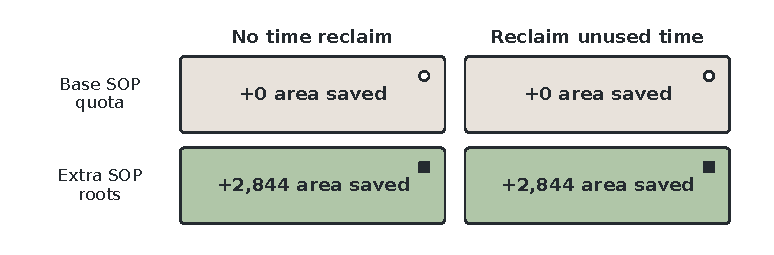
\includegraphics[width=.74\textwidth]{figures/r86_factorial_design.pdf}
\caption{Controlled R8.6 search-allocation experiment, run 1. The numbers denote aggregate area saved against the same fixed policy baseline, not program-runtime reductions. Hollow circles indicate the base quota and filled squares the extra-root treatment; color is redundant. Increased SOP root coverage matters on these 50 cases; recovering extra nominal time without changing quota does not. R8.6 differs from R10.0's later sequential follow-up.}
\label{fig:factorial}
\end{figure*}

\subsection{R9.0 feasibility safeguards and the R9.1 choice}
R9.0 introduced an exact short-budget streaming path for simple/affine high-dimensional functions and retained a safer default without committing to expensive speculative search. R9.1 then asked a different question: given a completed, legal network, where should the last small search budget go? A template-library approach improved \emph{more cases} but yielded only 663 aggregate area units, whereas a repeated SOP cut pass improved fewer cases but yielded 1,587 under the archived controlled comparison. A repeated Shannon pass was another option. The result distinguishes improvement frequency from improvement magnitude: the algorithm's objective is priced total area under validity constraints, not the count of cases with any positive change. R10.0 promotes the repeat-SOP choice to the plain-executable default; it does \emph{not} invent a new truth-signature algorithm.

\subsection{The last pass is a guarded, sequential transformation}
Let \(G_0\) be the already selected incumbent after the earlier work and \(t\) the elapsed program time. The last pass is admitted only if \(B\ge1000\) ms, \(G_0\) is valid and on target, and
\begin{equation}
 b_{\mathrm{last}}=\min\{90\,\mathrm{ms},\,0.06B,\,0.82B-t\}\ge8\,\mathrm{ms}.
\label{eq:lastbudget}
\end{equation}
The default setting examines at most 160 priority-selected roots through an additional SOP resynthesis pass, acting on \(G_0\) rather than restarting from the original R8.6 input. If the completed output \(G_1\) is valid, target-feasible and \(A(G_1)<A(G_0)\), it replaces \(G_0\); otherwise \(G_0\) remains the output. The template library and repeated Shannon remain opt-in experimental modes. The retained graph's exact cost is re-evaluated; local surrogate savings alone never authorize promotion. Here ``valid'' denotes the typed graph's structural and indexing checks, not an independent proof of its truth-table semantics on every pass. The semantics rely on exact local construction and are tested separately by the course evaluator and additional independent checks.

\begin{lemma}[Non-regression of the final pass relative to its own incumbent]
Assume correct full-network metric computation and serialization. If the final repeat-SOP pass returns normally, its selected output \(G_{\rm out}\) obeys \(A(G_{\rm out})\le A(G_0)\), and any accepted replacement obeys \(D(G_{\rm out})\le\Delta\).
\end{lemma}
\begin{IEEEproof}
If the pass is skipped or rejected, the incumbent is unchanged and the area equality holds. If accepted, the explicit test requires validity, \(D(G_1)\le\Delta\), and \(A(G_1)<A(G_0)\). These cases exhaust the final selection. The lemma makes no assertion about an unrelated execution of an older executable, because earlier clock-bounded searches can select different incumbents.
\end{IEEEproof}

A critical distinction is therefore that two passes are \emph{not additive independent improvements}. The R8.6 branches compete against one baseline; the R10 pass changes a graph previously altered by the winning branch. Its opportunities depend on fanout, removed nodes and the newly exposed cuts. A separate fixed-network experiment even found both orders of SOP/Shannon passes preferable on different saved graphs \cite{stage2trial}. This is why the final algorithm records strict global acceptance instead of predicting improvements from isolated local cover counts.

\paragraph{Why the early and late safety rules are different.}
The initial candidate portfolio may need to keep a valid circuit even when it has not yet reached \(\Delta\); Eq.~\eqref{eq:rank} therefore ranks target violations first. After a target-feasible incumbent has been produced, speculative cut searches are optional: the R8.6 area controller admits only feasible full graphs under Eq.~\eqref{eq:controller-eligible}, while the R10 SOP follow-up insists on strict area reduction. Thus the code gradually tightens its admission rules as a usable output becomes available. This explains the safeguard's role without incorrectly describing the entire program as a single monotone area-only greedy search.

\paragraph{Why pass order cannot be treated as a commutative optimization.}
Even under strict function-preserving replacement, the two search operators need not commute as graph transformations: $P(H(G))$ and $H(P(G))$ compute the same Boolean outputs when all local rewrites are correct, yet they may expose different candidate cuts, share different intermediate nodes, and produce different areas. A separate fixed-incumbent probe preserved the initial network and a 160-root allowance per pass on six deliberately selected graphs. SOP then Shannon was better on three; Shannon then SOP was better on one; two tied. On Stage 2 case 005 the former obtained area 102,471 versus 102,716, while on case 003 the latter obtained 15,575 versus 15,585. These are controlled \emph{counterexamples to universal order independence}, not a representative estimate of the probability that one order wins. They explain the conservative adopted rule: select fully measured completed candidates and accept a guarded additional pass only for strict area improvement, rather than assume that every additional search composes additively \cite{stage2trial}.



\section{Evaluation on the Released Project Instances}
\label{sec:evaluation}
\subsection{Protocol and reproducibility boundaries}
The historical research comparison uses the \emph{actually submitted} Stage 1 Z1 implementation, the independently frozen J51 research solver, and R10.0 on the same 25 Stage 1 and 25 Stage 2 released cases, under one WSL evaluator environment and identical C++17 optimization flags. Two matched runs reversed method order to expose some order sensitivity. The source and input hashes were retained in the archived case table. All case-level figures reported here from this batch can be recomputed from \texttt{data/matched\_case\_metrics.csv}, with the complete Z1/R10 first-run table in Appendix~\ref{sec:appendix}. A separate original R10 official-feedback archive contains two additional per-bank repetitions.

\begin{table}[!t]
\centering\caption{Matched 50-case comparison, one paired repeat. Area is summed only over PASS cases; J51's failed Stage 2 case makes its two-bank total \emph{incomparable} to two 50/50-pass totals. Times are medians within each bank.}
\label{tab:matched}
\footnotesize
\begin{tabular}{llrrrr}
\toprule
Bank & Program & PASS & Target & Area & Med. ms\\
\midrule
\multirow{3}{*}{Stage 1} & Z1 &25/25&25/25&589,023&605.75\\
 & J51 &25/25&25/25&529,014&61.36\\
 & R10 &25/25&25/25&525,582&193.70\\
\midrule
\multirow{3}{*}{Stage 2} & Z1 &25/25&25/25&555,221&603.78\\
 & J51 &24/25&24/25&506,754\textsuperscript{a}&36.93\\
 & R10 &25/25&25/25&493,965&130.71\\
\bottomrule
\end{tabular}
\vspace{1mm}\parbox{.98\columnwidth}{\scriptsize \textsuperscript{a}Only the 24 passed J51 cases are counted; its case 016 with a 100-ms limit is FAIL. No 50-case J51 area sum is claimed.}
\end{table}

\subsection{The main Stage 1--Stage 2 result is distributional}
In matched run 1, Z1 and R10 both pass and meet all 50 delay targets, with aggregate areas \(1{,}144{,}244\) and \(1{,}019{,}547\), respectively. The saved area is \(124{,}697\), or \(10.90\%\) relative to the Z1 baseline. On the first bank the decrease is \(63{,}441\); on the second it is \(61{,}256\). In matched run 2 the corresponding totals are \(1{,}145{,}191\) and \(1{,}019{,}883\), a decrease of \(125{,}308\). Both versions remain 50/50 PASS and 50/50 target-met in both repeats. Recomputing the signed differences case by case shows the \emph{same 18 positive and 32 negative cases} in both repeats; the sign never flips, although the gain magnitudes change slightly on three cases. This is stronger evidence for the \emph{observed distributional pattern} than an aggregate total alone, but it is still only a two-repeat result on the released inputs. These observations support robust public-case aggregate savings across the two measured orders, not a universal per-input superiority statement.

Indeed, R10 uses \emph{more} area than Z1 on 32 of the 50 first-run cases and \emph{less} on only 18. The 18 positive contributions sum to \(160{,}696\), whereas the 32 regressions cost \(35{,}999\), leaving \(124{,}697\) net savings. The median individual area difference is $-54.5$ units (Z1 minus R10), favoring Z1 on a typical ranked instance. The same 9-benefit/16-regression split appears separately in each 25-case bank: the Stage 1 bank saves $81{,}805$ but gives back $18{,}364$; the Stage 2 bank saves $78{,}891$ and gives back $17{,}635$. These complementary signed contributions, rather than a universal per-case gain, produce the two bank-level totals. Figure~\ref{fig:heterogeneity} makes the apparent paradox explicit: the objective weights the \emph{magnitude} of savings, not the number of winning instances. The largest single improvement, Stage 2 case 005, saves \(39{,}516\), while Stage 2 case 002 costs \(8{,}003\) more. The three largest positive cases together contribute \(94{,}004\) units, or about \(58.5\%\) of the \(160{,}696\) gross favorable contribution. Those examples must both remain visible in any defensible comparison. Every circuit in the paired Z1/R10 sample meets its target; area comparisons therefore do not conceal a FAIL or deadline miss.
\begin{figure*}[!t]
\centering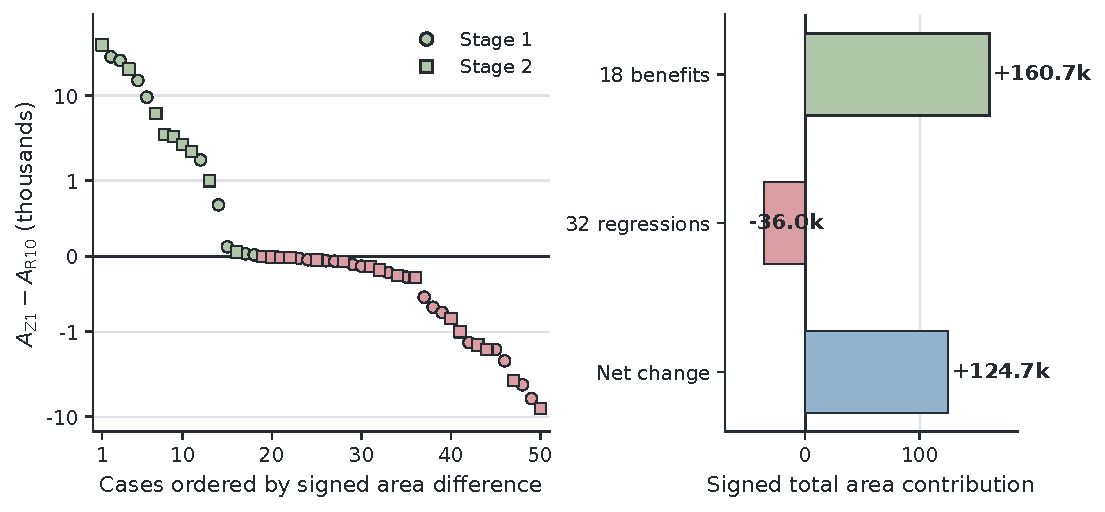
\includegraphics[width=.99\textwidth]{figures/area_case_heterogeneity.pdf}
\caption{Matched repeat 1, all 50 released cases. Left: signed area difference (Z1 minus R10), ranked by benefit, with a symmetric-log vertical axis to make small regressions visible alongside very large savings. Symbol shape distinguishes the bank, and fill distinguishes the sign. Right: the separate beneficial and adverse area contributions explain why 18 wins nevertheless deliver a positive aggregate saving. Zero would mean equal physical area; no equality occurs in this pairing.}
\label{fig:heterogeneity}
\end{figure*}

\subsection{Runtime and target-delay comparison}
Within matched repeat 1, Z1 has median synthesis times \(605.75\) and \(603.78\) ms on the two banks; R10's corresponding medians are \(193.70\) and \(130.71\) ms. On 49 of 50 cases R10 runs faster than Z1 in that batch; the exception is Stage 1 case 024, where R10 takes 674.605 ms longer. A common 50-case median, 605.26 ms for Z1 versus 164.80 ms for R10, is descriptive of that run and must not be mistaken for a portable machine-independent speedup. The comparison reflects \emph{different programs with different search schedules}; it is not an isolated measurement of the typed-DAG implementation or of cut-search overhead. Also, median synthesis time summarizes the center of the tested distribution, not the ability to finish every individual case under its own stated limit. Figure~\ref{fig:runtime} displays the full empirical runtime distribution rather than only two summary statistics. In contrast, J51 is usually faster than R10 when it completes, but it fails Stage 2 case 016 under the 100-ms limit. For that case the observed Z1 and R10 runtimes are 64.395 and 29.696 ms, with areas 1,647 and 1,781 and delays 38 and 36. Thus R10's successful deployment is not reducible to minimum runtime \emph{or} minimum area alone.
\begin{figure}[!t]
\centering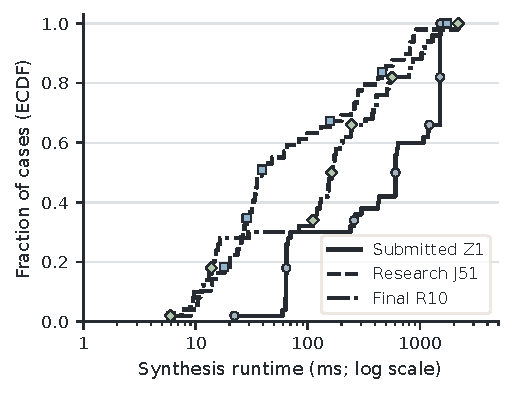
\includegraphics[width=\columnwidth]{figures/matched_runtime_ecdf.pdf}
\caption{Case-wise empirical CDF of synthesis time for the three methods in matched repeat 1 (50 Z1 and R10 PASS runtimes; 49 J51 PASS runtimes; log horizontal axis). The failed J51 case has no valid runtime entry and is not assigned an artificial zero. Linestyles and markers distinguish series in grayscale; traces are not confidence bands.}
\label{fig:runtime}
\end{figure}

Both Z1 and R10 meet all target delays, so their full-network time values are feasible but not monotonically ordered. Across 50 first-run cases, R10 improves the circuit delay in 27 cases, increases it in 18, and ties it in 5. The sum of delays is 2,399 for Z1 and 2,382 for R10, but this \emph{sum is not a single circuit's delay} and is not an official grading metric. The defensible conclusion is per-instance feasibility plus the observed distribution of delays. Since the project scoring weights area, delay, and runtime but does not publish a numerical formula, the report makes no numerical claim about final grade.

\subsection{The role of J51 in the comparison}
J51 materially improved the first-batch area relative to the submitted Z1 baseline: the matched Stage 1 area is 529,014 versus 589,023, while both pass all 25. The independent Stage 1 research therefore belongs in the technical history and not merely a footnote. It also exposes why a single attractive Stage 1 metric cannot replace Stage 2 validation: on the second bank J51 passes only 24/25. The failed case is retained explicitly, and the area sum of its passed cases is \emph{not} merged with its first-bank sum to manufacture a 50/50 comparison. R10 combines similar representation/typed-DAG ideas with new time-safe defaults and cut search, accepting some per-case tradeoffs to achieve complete observed validity.

\section{Final Team Integration}\label{sec:integration}

The archive \texttt{Final\_Submission\_by\_Zeyun\_DU} pins commit \texttt{59e3350} and records the source, header, and evaluator identities \cite{stage2integration}. It is the planned final team version. The integrated solver adapts Round 5.1 BDD, cover and typed-DAG mapping and the R10.0 four-leaf cut mapper. Its controller searches variable orders, selects complete shared-output circuits, reserves one integer unit of delay when the target exceeds one, and can rebuild late outputs from exact cofactors and covers. The nominal main search allowance for positive limits is the smaller of \(0.45L\) and 3.3 seconds, where \(L\) is the per-case time limit. Postprocessing and output consume additional time. Earlier instrumented experiments isolate cut rewriting and shared-factor effects on fixed incumbents. The full version comparison measures a combined change in mapping, selection, timing recovery and budgets.

\begin{table}[!t]
\centering\small
\caption{Matched integration benchmark. Each repeat covers both banks (50 cases). Columns give evaluator PASS count and target count, total weighted area, and the sum of evaluator-reported synthesis durations.}
\label{tab:integration}
\begin{tabular}{@{}rlrrr@{}}
\toprule
Run & Method & PASS / target & Area & s\\
\midrule
\IntegrationRows
\bottomrule
\end{tabular}
\end{table}

Table~\ref{tab:integration} uses two sequential repeats on one WSL2 host, a common GCC build configuration, and the same course evaluator and released inputs for all four solvers. The integrated circuits were independently replayed for every assignment in both repeats, with at least one delay unit of slack on every input. Integrated Final saved about 22.6\% area relative to Z1 and 14.4\% relative to R10.0 in each repeat. Its median per-case synthesis time ratio relative to R10.0 was 2.316 and 2.262 across the two repeats. The integration audit gives the corresponding ratios of total time, delay statistics, maximum use of case time limits and peak process RSS from separate direct runs.

The upstream acceptance batch reported weighted areas of 884,234, 876,694 and 876,694 and a maximum runtime of 49.7\% of a case limit. The earlier upstream cuts comparison recorded 869,773 for its integrated snapshot. The pinned source introduced changes after that snapshot. The archive preserves both casewise records and the in-run experimental controls.

\section{What the Controlled Postprocessing Experiments Establish}
\label{sec:ablation}
\subsection{R9.0 versus R10.0: sparse marginal gains}
The R10.0 original feedback archive also contains the frozen R9.0 source executed against R10 under the same archived cases. In first-run comparisons, the repeated SOP pass reduces aggregate area by \(1{,}587\) across 50 cases, affecting only eight instances; 42 are unchanged and none loses area, with delays unchanged. The largest single gain is \(752\), or 47.39\% of the total, while the smallest positive gain is only \(2\). Figure~\ref{fig:sparse} separates the eight actual discoveries from the 42 unchanged outputs. This modest improvement is still relevant to the final design because the optional search has a fixed root quota and periodic clock checks, and it never replaces the current incumbent without a strict full-graph reduction. These controls limit attempted work but do not constitute a universal hard runtime bound. It would be misleading to call the last pass a transformation that improves most input functions.
\begin{figure}[!t]
\centering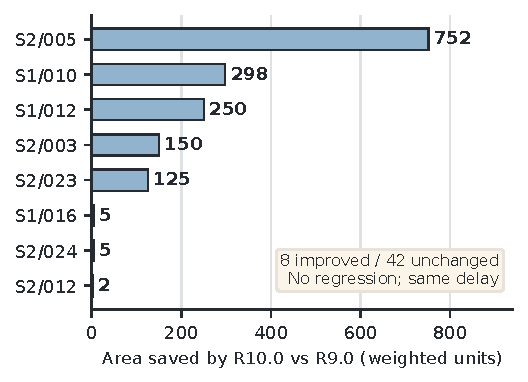
\includegraphics[width=\columnwidth]{figures/last_pass_sparse_benefit.pdf}
\caption{Positive per-case savings of the default R10.0 additional SOP pass relative to frozen R9.0, from their archived first-run comparison. The eight nonzero values sum to 1,587; 42 others are equal. R10.0 does not universally outperform a separately timed R9.0 run by theorem; this is a measured paired result.}
\label{fig:sparse}
\end{figure}

\subsection{Why the accepted search budget belongs to the final algorithm}
R10.1 tested reduced root caps and smaller nominal last-pass allowances. Against the R10.0 baseline area of 1,019,547 over the 50 public cases, root cap 40 yielded 1,020,555; root cap 80 yielded 1,020,149; a 45-ms time budget yielded 1,019,788. These regressions are \(1{,}008\), \(602\), and \(241\) area units, respectively. Reported runtime differences across the two repeat orders were not uniformly favorable to the nominally smaller searches \cite{stage2trial}. Together with the earlier R8.6 factorial, this gave a concrete stopping rule: preserve the observed area gain from prioritized search and avoid further tuning without evidence of a stable deployment benefit. An additional template library remained a valid experimental idea but had a weaker aggregate area outcome than repeat-SOP in the tested workload.

A native paired comparison clarifies the \emph{joint} decision rather than treating lower area and lower runtime as unrelated version statistics. Figure~\ref{fig:final-policy} reports the positive area penalty of each alternate policy relative to frozen R10.0, together with its median \emph{paired} synthesis-runtime ratio. The same original 50 cases are observed over two repetitions for each policy (100 matched observations); the summed area differences are therefore halved to obtain a 50-case equivalent. Disabling the extra SOP pass is faster (ratio $0.942$) but costs $1{,}587$ area units. Limiting it to 40 or 80 roots loses $1{,}008$ or $602$ units, respectively, with much smaller observed time savings (ratios $0.987$ and $0.988$). A 45-ms allowance loses $241$ units, and its median ratio is $1.009$, not an improvement. These observations support retaining a modest optional search budget rather than asserting that either ``more time'' or ``fewer roots'' always wins.
\begin{figure*}[!t]
\centering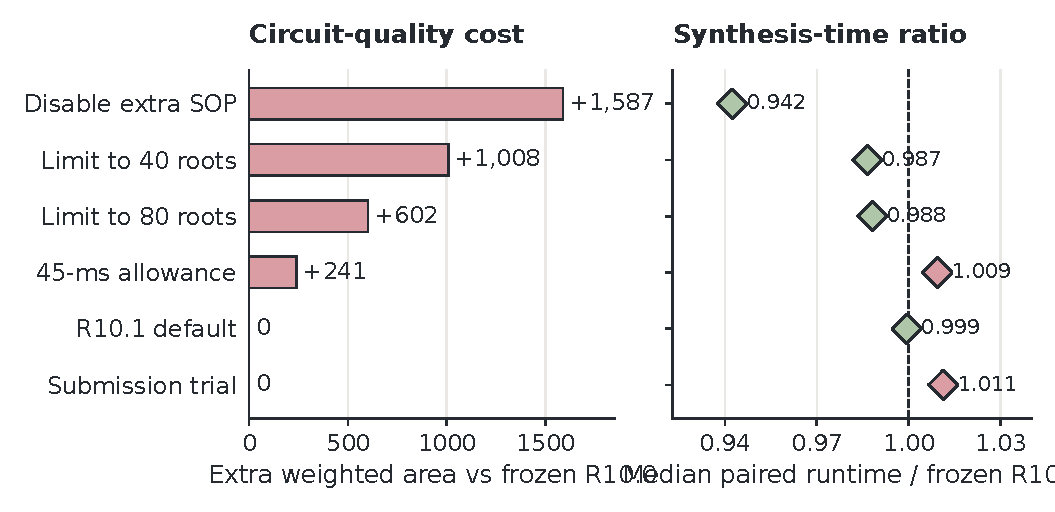
\includegraphics[width=.90\textwidth]{figures/final_policy_tradeoff.pdf}
\caption{Source-native R10.1 controlled policy comparison relative to frozen R10.0: left, positive extra total weighted area is worse; right, ratios below 1 indicate lower median paired synthesis runtime. Values correspond to 100 matched case--repeat observations per policy normalized to 50-case area totals. This is a conditional operating-point comparison, not a cross-round causal frontier.}
\label{fig:final-policy}
\end{figure*}


\subsection{Interpretation of negative results}
The experiments also explain why the final policy is selective rather than maximally exhaustive. Increasing time alone did not help the fixed-quota R8.6 treatment, whereas exposing additional SOP roots did; this identifies \emph{candidate coverage}, rather than nominal wall time, as the observed limitation of that treatment. The sparse R9.0--R10.0 gains show that a second pass can be worthwhile without often finding a better circuit. Neither result supports unlimited search: quotas can terminate before a time allowance is consumed, and clock-triggered checks can change which candidate finishes. The resulting design spends additional work only after a feasible incumbent exists and retains a new network only after whole-DAG evaluation.

\section{Correctness, Resource Boundaries, and Reproduction}
\begin{proposition}[Conditional end-to-end functional correctness]
Assume the initial mapped netlist implements the complete input table, each subsequent transformation emits legal topologically ordered gates and preserves the Boolean function at every replaced boundary, and the final serializer retains all primary outputs and their live ancestors. Then any normally returned netlist implements every output of the original truth table. If a target-feasible incumbent has been reached and each subsequent optional selection retains the incumbent unless its replacement is target-feasible, the returned circuit also meets \(\Delta\).
\end{proposition}
\begin{IEEEproof}
The initial construction provides the induction base. A valid local transformation changes no Boolean signal visible outside its replacement boundary, as established by the cut-equivalence proposition or the exact Shannon/algebraic identity used. Composition of finitely many such transformations preserves the output vector. Rebuilding and reachability pruning change identifiers and discard only nodes unused by every output, so they leave each output function unchanged. Once a target-feasible incumbent exists, the optional selection rule either keeps it or replaces it with a complete network whose measured delay is at most \(\Delta\); induction across selections proves feasibility of the survivor.
\end{IEEEproof}
The proposition states \emph{algorithmic invariants under explicit implementation assumptions}. In particular, it neither guarantees that a feasible initial circuit is discovered within every stated resource limit nor proves the C++ implementation free from defects. The short-budget/low-memory specialized paths are separately justified by exhaustive table recognition and checked construction; when the RAM fallback cannot solve an instance, the program can return failure rather than a speculative circuit.

\subsection{Implementation-level verification}
The propositions above establish why the specified transformations preserve functionality and, under stated timing conditions, delay feasibility. They do not validate every parser branch, graph index, or time-dependent policy in the compiled program. We therefore separate \emph{mathematical invariants} from \emph{implementation evidence}: independent netlist checks verify emitted gate legality and function values, while evaluator results establish per-case correctness, target feasibility, and observed execution behavior. Full-DAG area and delay recomputation is an admission check, not an independent proof that an arbitrarily constructed replacement has the correct Boolean function.

The implementation was separately compiled with GCC/C++17 and passed 20 independent exhaustive small-function source-run checks across Z1 and R10 (five functions, two runtime settings, both solvers). The 18-input synthetic affine stream path was also exercised and its output independently checked across all \(2^{18}\) assignments. In addition, two original archived R10 feedback rounds each report 25/25 PASS and 25/25 target-met in both released banks (original per-bank area sums: 525,582 and 493,965). These are differentiated as current smoke tests, archived course-evaluator evidence, and mathematical correctness claims, rather than being described as one universal formal proof.

\subsection{Resource guards are useful but not hard bounds}
Reading a complete \(m\)-output truth table already requires \(\Omega(m2^n)\) bits of input work. Fixed-order BDDs can have exponential worst-case size. The program's 65/77/82-percent admission points, root caps, and periodic deadline checks reduce risk from optional searches but are not a hard asynchronous interruption guarantee for arbitrary positive runtime limits. The conservative RAM admission logic is likewise not a theorem bounding peak resident memory. These qualifications matter for hidden-test claims; they do not undo the measured 50-case PASS outcomes. R10's result should therefore be described as an empirically successful, resource-aware heuristic synthesis system, not as a universally optimal or real-time synthesis algorithm.

\subsection{Provenance and reproducible comparisons}
The historical investigation uses the frozen R10.0 \texttt{synth.cpp} with SHA-256 \texttt{8c863f1a\ldots f5b15d}. The submitted Stage 1 source has SHA-256 \texttt{cd31f7d2\ldots 584550}. The source and header snapshots were audited together, and the archived evidence collector's 26 original materials matched its recorded file hashes. The integrated archive includes a source manifest, the local run environment and a numerical verification script. Both benchmark protocols use the repository's existing copies of the course evaluator and truth tables.

\section{Individual Contributions, Teamwork, and AI Assistance}
The project began with two independent Stage 1 investigations. Zeyun Du produced the submitted Stage 1 solution. Jincan Li developed and documented a separate R1--R6.1 investigation, including the R5.1 freeze and exploratory cut rewriting. Jincan led the independent Stage 2 algorithm design, implementation, evaluation and selection of R10.0. Zeyun coordinated the Stage 2 team integration and validation and set its public area and timing objectives. Its source credits the J51 modules and the R10.0 cut mapper. The upstream integration report credits Codex with implementing timing rescue and assisting with release verification and packaging \cite{stage2integration}.

Generative-AI systems assisted substantially with C++ implementation, verification scripts, mathematical exposition, experiment orchestration and document drafting. The student-led role included choosing hypotheses and comparison standards, executing the evaluator, questioning suggested optimizations, rejecting unprofitable branches, auditing results, and deciding what to freeze. Code hashes, raw evaluator feedback, independent correctness checks and retained negative results allow specific claims to be reviewed, but no statement of unaided code authorship or universal validation is made. Both students remain responsible for the accuracy of the report and any final submission.

\section{Conclusion}
Exact functional representations construct a starting circuit, and the shared DAG determines weighted area and critical-path delay. Bounded four-leaf resynthesis exposes alternative realizations under a finite search budget. In its historical matched tests, R10 meets all 50 targets and saves about 10.9\% aggregate area versus submitted Stage 1. The final team archive evaluates integrated mapping, timing recovery and scheduling together under a new matched protocol. Its public results support the planned release, with observed area, timing slack and resource use documented separately.

\bibliographystyle{IEEEtran}
\bibliography{references}

\clearpage\onecolumn
\appendices
\section{Casewise Stage 1--Stage 2 Evaluation}\label{sec:appendix}
Table~\ref{tab:casewise} gives the first paired repeat of the historical comparison between submitted Stage 1 (Z1) and the R10.0 research freeze. Both methods pass and meet the target on all 50 entries. The explicit "P/P" column indicates Z1 PASS / R10 PASS. The case-level PASS flags, area, delay and measured synthesis runtime come from the hash-tracked matched-case table. The second matched repeat and the independent J51 observations, including J51's Stage 2/016 FAIL, are preserved in \texttt{data/matched\_case\_metrics.csv}.
% Generated by build_casewise.py from archived matched_case_metrics.csv.
\newcommand{\PhaseCMatchedRows}{%
1 & Z1 & 1,127,450 & 37.151 & 63.04\% \\%
1 & J51 & 1,037,549 & 8.663 & 97.92\% \\%
1 & R10.0 & 1,019,547 & 14.736 & 21.95\% \\%
1 & Integrated & 872,813 & 32.350 & 51.94\% \\%
2 & Z1 & 1,127,196 & 36.954 & 67.52\% \\%
2 & J51 & 1,037,549 & 9.419 & 96.93\% \\%
2 & R10.0 & 1,019,547 & 15.047 & 23.62\% \\%
2 & Integrated & 872,919 & 32.243 & 51.95\% \\%
}
\newcommand{\PhaseCCasewise}{%
\begingroup\footnotesize
\setlength\tabcolsep{4pt}
\begin{longtable}{@{}lr*{4}{rrr}@{}}
\caption{Matched repeat 1, Stage 1. All four methods passed and met all 25 targets.}\\
\toprule
 & & \multicolumn{3}{c}{Z1} & \multicolumn{3}{c}{J51} & \multicolumn{3}{c}{R10.0} & \multicolumn{3}{c}{Integrated Final} \\
\cmidrule(lr){3-5}\cmidrule(lr){6-8}\cmidrule(lr){9-11}\cmidrule(lr){12-14}
Case & Target & Area & Delay & ms & Area & Delay & ms & Area & Delay & ms & Area & Delay & ms \\
\midrule
\endfirsthead
\toprule
 & & \multicolumn{3}{c}{Z1} & \multicolumn{3}{c}{J51} & \multicolumn{3}{c}{R10.0} & \multicolumn{3}{c}{Integrated Final} \\
\cmidrule(lr){3-5}\cmidrule(lr){6-8}\cmidrule(lr){9-11}\cmidrule(lr){12-14}
Case & Target & Area & Delay & ms & Area & Delay & ms & Area & Delay & ms & Area & Delay & ms \\
\midrule
\endhead
\bottomrule
\endlastfoot
001 & 77 & 55,838 & 76 & 1508.60 & 61,952 & 62 & 449.60 & 61,952 & 62 & 721.91 & 53,955 & 73 & 1915.20 \\
002 & 61 & 28,481 & 38 & 1503.71 & 18,897 & 60 & 137.69 & 18,888 & 60 & 276.11 & 14,765 & 60 & 616.38 \\
003 & 64 & 20,033 & 55 & 1503.36 & 24,251 & 56 & 171.74 & 24,235 & 56 & 337.07 & 14,983 & 55 & 799.60 \\
004 & 57 & 3,209 & 56 & 388.36 & 4,550 & 47 & 16.03 & 4,546 & 47 & 129.41 & 3,211 & 55 & 113.81 \\
005 & 36 & 590 & 34 & 61.47 & 700 & 31 & 21.31 & 700 & 31 & 6.86 & 590 & 34 & 26.83 \\
006 & 60 & 5,218 & 60 & 526.33 & 5,962 & 46 & 20.33 & 5,962 & 46 & 148.61 & 5,269 & 59 & 140.93 \\
007 & 89 & 106,573 & 85 & 1509.13 & 78,042 & 71 & 581.94 & 78,042 & 71 & 945.29 & 78,042 & 71 & 2337.59 \\
008 & 62 & 6,437 & 59 & 602.44 & 8,637 & 50 & 27.55 & 8,637 & 50 & 170.67 & 6,544 & 61 & 210.58 \\
009 & 59 & 12,963 & 57 & 603.05 & 14,584 & 46 & 45.49 & 14,579 & 46 & 200.20 & 14,584 & 46 & 332.94 \\
010 & 61 & 4,792 & 30 & 1155.59 & 4,712 & 32 & 104.41 & 3,037 & 61 & 220.33 & 2,752 & 60 & 175.97 \\
011 & 40 & 436 & 33 & 60.02 & 464 & 33 & 22.20 & 464 & 33 & 5.87 & 436 & 33 & 24.42 \\
012 & 40 & 4,442 & 25 & 319.52 & 5,359 & 25 & 19.07 & 3,763 & 40 & 142.27 & 3,903 & 39 & 98.29 \\
013 & 70 & 10,692 & 56 & 1145.51 & 11,252 & 60 & 70.74 & 11,234 & 60 & 185.90 & 9,232 & 60 & 352.31 \\
014 & 72 & 11,344 & 59 & 1502.56 & 11,662 & 61 & 227.89 & 11,622 & 61 & 340.18 & 11,120 & 61 & 577.32 \\
015 & 81 & 33,490 & 80 & 1504.08 & 33,374 & 64 & 278.10 & 33,366 & 64 & 449.52 & 31,565 & 63 & 1450.14 \\
016 & 47 & 2,172 & 47 & 235.84 & 2,149 & 40 & 11.55 & 2,140 & 40 & 103.12 & 2,149 & 40 & 61.65 \\
017 & 25 & 393 & 25 & 62.94 & 440 & 22 & 3.59 & 440 & 22 & 3.62 & 383 & 22 & 47.19 \\
018 & 32 & 1,167 & 32 & 63.04 & 1,232 & 31 & 6.84 & 1,232 & 31 & 6.89 & 1,174 & 31 & 47.73 \\
019 & 73 & 4,594 & 69 & 1119.26 & 5,319 & 57 & 87.27 & 5,269 & 57 & 208.75 & 4,408 & 71 & 227.15 \\
020 & 35 & 634 & 35 & 62.61 & 766 & 30 & 21.75 & 766 & 30 & 7.97 & 645 & 34 & 28.59 \\
021 & 72 & 27,888 & 60 & 1504.57 & 28,104 & 60 & 314.29 & 28,104 & 60 & 478.11 & 27,084 & 61 & 1342.02 \\
022 & 34 & 1,044 & 32 & 62.86 & 1,320 & 31 & 26.65 & 1,320 & 31 & 11.22 & 1,082 & 31 & 41.46 \\
023 & 24 & 142 & 24 & 20.56 & 125 & 22 & 4.59 & 125 & 22 & 2.37 & 202 & 15 & 6.97 \\
024 & 83 & 139,590 & 67 & 1515.20 & 124,475 & 70 & 1310.98 & 124,473 & 71 & 1804.83 & 124,467 & 72 & 3027.88 \\
025 & 76 & 106,643 & 76 & 1510.92 & 80,686 & 60 & 588.28 & 80,686 & 60 & 915.78 & 80,679 & 60 & 2307.19 \\
\end{longtable}
\begin{longtable}{@{}lr*{4}{rrr}@{}}
\caption{Matched repeat 1, Stage 2. All four methods passed and met all 25 targets.}\\
\toprule
 & & \multicolumn{3}{c}{Z1} & \multicolumn{3}{c}{J51} & \multicolumn{3}{c}{R10.0} & \multicolumn{3}{c}{Integrated Final} \\
\cmidrule(lr){3-5}\cmidrule(lr){6-8}\cmidrule(lr){9-11}\cmidrule(lr){12-14}
Case & Target & Area & Delay & ms & Area & Delay & ms & Area & Delay & ms & Area & Delay & ms \\
\midrule
\endfirsthead
\toprule
 & & \multicolumn{3}{c}{Z1} & \multicolumn{3}{c}{J51} & \multicolumn{3}{c}{R10.0} & \multicolumn{3}{c}{Integrated Final} \\
\cmidrule(lr){3-5}\cmidrule(lr){6-8}\cmidrule(lr){9-11}\cmidrule(lr){12-14}
Case & Target & Area & Delay & ms & Area & Delay & ms & Area & Delay & ms & Area & Delay & ms \\
\midrule
\endhead
\bottomrule
\endlastfoot
001 & 41 & 2,102 & 32 & 619.76 & 2,086 & 32 & 29.18 & 2,046 & 32 & 94.28 & 1,662 & 39 & 509.85 \\
002 & 86 & 50,694 & 77 & 1505.72 & 58,697 & 68 & 599.53 & 58,697 & 68 & 872.85 & 50,225 & 85 & 2375.38 \\
003 & 65 & 19,105 & 39 & 1503.05 & 19,494 & 39 & 249.91 & 15,623 & 65 & 426.45 & 12,244 & 63 & 612.63 \\
004 & 42 & 744 & 26 & 621.40 & 932 & 23 & 29.31 & 928 & 23 & 76.38 & 660 & 31 & 519.41 \\
005 & 69 & 126,127 & 40 & 1509.18 & 112,221 & 40 & 667.51 & 102,889 & 68 & 1011.91 & 60,744 & 68 & 2285.81 \\
006 & 56 & 5,076 & 48 & 601.81 & 8,834 & 49 & 28.94 & 8,814 & 49 & 136.95 & 5,138 & 48 & 228.73 \\
007 & 52 & 992 & 44 & 62.33 & 1,250 & 52 & 15.66 & 1,250 & 52 & 9.07 & 991 & 44 & 47.37 \\
008 & 36 & 932 & 36 & 61.84 & 952 & 30 & 26.36 & 952 & 30 & 8.02 & 878 & 35 & 32.99 \\
009 & 40 & 942 & 35 & 62.08 & 1,169 & 25 & 10.07 & 1,169 & 25 & 6.83 & 861 & 33 & 35.19 \\
010 & 23 & 230 & 21 & 61.99 & 235 & 22 & 2.47 & 235 & 22 & 2.46 & 214 & 21 & 29.00 \\
011 & 79 & 55,112 & 79 & 1505.75 & 52,463 & 62 & 494.34 & 52,463 & 62 & 761.64 & 38,420 & 78 & 1708.64 \\
012 & 43 & 3,320 & 38 & 417.30 & 4,153 & 38 & 43.51 & 4,143 & 38 & 115.35 & 3,352 & 39 & 122.05 \\
013 & 78 & 114,280 & 64 & 1507.81 & 115,734 & 66 & 822.10 & 115,706 & 66 & 1337.41 & 82,364 & 68 & 2668.31 \\
014 & 83 & 65,808 & 70 & 1509.68 & 62,535 & 66 & 357.59 & 62,511 & 66 & 639.07 & 62,535 & 66 & 2193.03 \\
015 & 55 & 6,652 & 55 & 602.74 & 7,656 & 48 & 29.90 & 7,652 & 48 & 136.79 & 5,770 & 46 & 227.41 \\
016 & 42 & 1,647 & 38 & 62.39 & 1,781 & 36 & 97.92 & 1,781 & 36 & 21.95 & 1,542 & 37 & 46.51 \\
017 & 57 & 12,456 & 48 & 603.13 & 14,188 & 49 & 58.79 & 14,154 & 49 & 148.46 & 11,192 & 52 & 330.23 \\
018 & 42 & 660 & 42 & 61.61 & 709 & 42 & 5.87 & 709 & 42 & 5.74 & 700 & 40 & 26.42 \\
019 & 35 & 641 & 33 & 61.63 & 711 & 28 & 16.84 & 711 & 28 & 6.83 & 598 & 33 & 24.36 \\
020 & 49 & 2,638 & 40 & 253.36 & 2,922 & 39 & 14.56 & 2,918 & 39 & 101.59 & 2,146 & 42 & 59.55 \\
021 & 70 & 43,078 & 44 & 1504.29 & 22,590 & 69 & 204.22 & 22,576 & 69 & 346.84 & 22,216 & 69 & 843.56 \\
022 & 33 & 776 & 27 & 61.88 & 794 & 28 & 29.07 & 794 & 28 & 9.14 & 787 & 28 & 37.67 \\
023 & 40 & 2,902 & 23 & 233.53 & 2,986 & 25 & 12.37 & 1,904 & 40 & 112.30 & 2,300 & 39 & 67.11 \\
024 & 63 & 9,082 & 61 & 602.09 & 6,910 & 52 & 24.39 & 6,873 & 52 & 159.73 & 6,108 & 62 & 209.56 \\
025 & 80 & 12,649 & 72 & 1503.37 & 6,533 & 73 & 222.46 & 6,467 & 73 & 364.94 & 5,942 & 73 & 798.77 \\
\end{longtable}
\begin{longtable}{@{}lr*{4}{rrr}@{}}
\caption{Matched repeat 2, Stage 1. All four methods passed and met all 25 targets.}\\
\toprule
 & & \multicolumn{3}{c}{Z1} & \multicolumn{3}{c}{J51} & \multicolumn{3}{c}{R10.0} & \multicolumn{3}{c}{Integrated Final} \\
\cmidrule(lr){3-5}\cmidrule(lr){6-8}\cmidrule(lr){9-11}\cmidrule(lr){12-14}
Case & Target & Area & Delay & ms & Area & Delay & ms & Area & Delay & ms & Area & Delay & ms \\
\midrule
\endfirsthead
\toprule
 & & \multicolumn{3}{c}{Z1} & \multicolumn{3}{c}{J51} & \multicolumn{3}{c}{R10.0} & \multicolumn{3}{c}{Integrated Final} \\
\cmidrule(lr){3-5}\cmidrule(lr){6-8}\cmidrule(lr){9-11}\cmidrule(lr){12-14}
Case & Target & Area & Delay & ms & Area & Delay & ms & Area & Delay & ms & Area & Delay & ms \\
\midrule
\endhead
\bottomrule
\endlastfoot
001 & 77 & 55,838 & 76 & 1508.73 & 61,952 & 62 & 464.94 & 61,952 & 62 & 742.46 & 53,955 & 73 & 1878.05 \\
002 & 61 & 28,481 & 38 & 1504.23 & 18,897 & 60 & 144.53 & 18,888 & 60 & 290.98 & 14,765 & 60 & 595.27 \\
003 & 64 & 20,033 & 55 & 1502.87 & 24,251 & 56 & 176.54 & 24,235 & 56 & 343.92 & 14,983 & 55 & 785.90 \\
004 & 57 & 3,209 & 56 & 369.22 & 4,550 & 47 & 16.74 & 4,546 & 47 & 135.80 & 3,211 & 55 & 115.30 \\
005 & 36 & 590 & 34 & 61.35 & 700 & 31 & 21.04 & 700 & 31 & 6.95 & 590 & 34 & 24.85 \\
006 & 60 & 5,218 & 60 & 522.68 & 5,962 & 46 & 20.00 & 5,962 & 46 & 152.34 & 5,269 & 59 & 140.73 \\
007 & 89 & 106,573 & 85 & 1508.78 & 78,042 & 71 & 607.45 & 78,042 & 71 & 980.73 & 78,042 & 71 & 2346.76 \\
008 & 62 & 6,437 & 59 & 602.09 & 8,637 & 50 & 27.68 & 8,637 & 50 & 169.14 & 6,544 & 61 & 218.05 \\
009 & 59 & 12,963 & 57 & 602.74 & 14,584 & 46 & 45.73 & 14,579 & 46 & 190.88 & 14,584 & 46 & 337.76 \\
010 & 61 & 4,792 & 30 & 1058.17 & 4,712 & 32 & 103.33 & 3,037 & 61 & 231.70 & 2,752 & 60 & 175.78 \\
011 & 40 & 436 & 33 & 55.21 & 464 & 33 & 23.45 & 464 & 33 & 5.89 & 436 & 33 & 23.54 \\
012 & 40 & 4,442 & 25 & 290.97 & 5,359 & 25 & 17.63 & 3,763 & 40 & 142.71 & 3,903 & 39 & 101.22 \\
013 & 70 & 10,692 & 56 & 1142.39 & 11,252 & 60 & 71.01 & 11,234 & 60 & 188.70 & 9,232 & 60 & 365.20 \\
014 & 72 & 11,344 & 59 & 1502.83 & 11,662 & 61 & 239.77 & 11,622 & 61 & 365.69 & 11,120 & 61 & 594.31 \\
015 & 81 & 33,490 & 80 & 1503.83 & 33,374 & 64 & 290.08 & 33,366 & 64 & 473.00 & 31,565 & 63 & 1490.58 \\
016 & 47 & 2,172 & 47 & 238.46 & 2,149 & 40 & 11.37 & 2,140 & 40 & 104.18 & 2,149 & 40 & 63.88 \\
017 & 25 & 393 & 25 & 62.55 & 440 & 22 & 3.64 & 440 & 22 & 3.65 & 383 & 22 & 47.11 \\
018 & 32 & 1,167 & 32 & 67.52 & 1,232 & 31 & 8.00 & 1,232 & 31 & 6.82 & 1,174 & 31 & 47.80 \\
019 & 73 & 4,594 & 69 & 1091.08 & 5,319 & 57 & 88.32 & 5,269 & 57 & 210.92 & 4,408 & 71 & 229.68 \\
020 & 35 & 634 & 35 & 61.95 & 766 & 30 & 21.13 & 766 & 30 & 8.07 & 645 & 34 & 29.57 \\
021 & 72 & 27,888 & 60 & 1504.10 & 28,104 & 60 & 323.66 & 28,104 & 60 & 460.49 & 27,084 & 61 & 1322.75 \\
022 & 34 & 1,044 & 32 & 62.34 & 1,320 & 31 & 29.17 & 1,320 & 31 & 10.21 & 1,082 & 31 & 42.72 \\
023 & 24 & 142 & 24 & 19.97 & 125 & 22 & 4.77 & 125 & 22 & 2.49 & 202 & 15 & 7.13 \\
024 & 83 & 139,590 & 67 & 1514.96 & 124,475 & 70 & 1356.75 & 124,473 & 71 & 1960.65 & 124,467 & 72 & 3072.72 \\
025 & 76 & 106,643 & 76 & 1520.46 & 80,686 & 60 & 610.71 & 80,686 & 60 & 910.71 & 80,679 & 60 & 2307.71 \\
\end{longtable}
\begin{longtable}{@{}lr*{4}{rrr}@{}}
\caption{Matched repeat 2, Stage 2. All four methods passed and met all 25 targets.}\\
\toprule
 & & \multicolumn{3}{c}{Z1} & \multicolumn{3}{c}{J51} & \multicolumn{3}{c}{R10.0} & \multicolumn{3}{c}{Integrated Final} \\
\cmidrule(lr){3-5}\cmidrule(lr){6-8}\cmidrule(lr){9-11}\cmidrule(lr){12-14}
Case & Target & Area & Delay & ms & Area & Delay & ms & Area & Delay & ms & Area & Delay & ms \\
\midrule
\endfirsthead
\toprule
 & & \multicolumn{3}{c}{Z1} & \multicolumn{3}{c}{J51} & \multicolumn{3}{c}{R10.0} & \multicolumn{3}{c}{Integrated Final} \\
\cmidrule(lr){3-5}\cmidrule(lr){6-8}\cmidrule(lr){9-11}\cmidrule(lr){12-14}
Case & Target & Area & Delay & ms & Area & Delay & ms & Area & Delay & ms & Area & Delay & ms \\
\midrule
\endhead
\bottomrule
\endlastfoot
001 & 41 & 2,102 & 32 & 613.76 & 2,086 & 32 & 33.58 & 2,046 & 32 & 89.36 & 1,768 & 39 & 477.69 \\
002 & 86 & 50,694 & 77 & 1505.93 & 58,697 & 68 & 763.75 & 58,697 & 68 & 874.74 & 50,225 & 85 & 2340.27 \\
003 & 65 & 19,105 & 39 & 1503.26 & 19,494 & 39 & 272.64 & 15,623 & 65 & 423.95 & 12,244 & 63 & 585.62 \\
004 & 42 & 744 & 26 & 617.96 & 932 & 23 & 34.67 & 928 & 23 & 68.83 & 660 & 31 & 519.50 \\
005 & 69 & 126,127 & 40 & 1506.62 & 112,221 & 40 & 851.85 & 102,889 & 68 & 1001.54 & 60,744 & 68 & 2274.74 \\
006 & 56 & 4,838 & 48 & 602.98 & 8,834 & 49 & 34.89 & 8,814 & 49 & 144.98 & 5,138 & 48 & 230.62 \\
007 & 52 & 992 & 44 & 61.47 & 1,250 & 52 & 17.45 & 1,250 & 52 & 9.38 & 991 & 44 & 47.10 \\
008 & 36 & 932 & 36 & 61.45 & 952 & 30 & 30.02 & 952 & 30 & 7.91 & 878 & 35 & 34.13 \\
009 & 40 & 942 & 35 & 62.18 & 1,169 & 25 & 10.52 & 1,169 & 25 & 6.99 & 861 & 33 & 35.61 \\
010 & 23 & 214 & 21 & 62.20 & 235 & 22 & 3.74 & 235 & 22 & 2.44 & 214 & 21 & 29.49 \\
011 & 79 & 55,112 & 79 & 1505.60 & 52,463 & 62 & 604.46 & 52,463 & 62 & 764.10 & 38,420 & 78 & 1682.60 \\
012 & 43 & 3,320 & 38 & 413.56 & 4,153 & 38 & 46.96 & 4,143 & 38 & 111.54 & 3,352 & 39 & 117.80 \\
013 & 78 & 114,280 & 64 & 1510.31 & 115,734 & 66 & 898.18 & 115,706 & 66 & 1297.34 & 82,364 & 68 & 2614.76 \\
014 & 83 & 65,808 & 70 & 1505.02 & 62,535 & 66 & 374.68 & 62,511 & 66 & 633.67 & 62,535 & 66 & 2182.67 \\
015 & 55 & 6,652 & 55 & 602.93 & 7,656 & 48 & 30.25 & 7,652 & 48 & 138.95 & 5,770 & 46 & 229.17 \\
016 & 42 & 1,647 & 38 & 62.27 & 1,781 & 36 & 96.93 & 1,781 & 36 & 23.62 & 1,542 & 37 & 47.53 \\
017 & 57 & 12,456 & 48 & 602.94 & 14,188 & 49 & 57.35 & 14,154 & 49 & 154.53 & 11,192 & 52 & 329.34 \\
018 & 42 & 660 & 42 & 62.45 & 709 & 42 & 5.89 & 709 & 42 & 5.95 & 700 & 40 & 25.94 \\
019 & 35 & 641 & 33 & 61.52 & 711 & 28 & 17.50 & 711 & 28 & 6.87 & 598 & 33 & 26.41 \\
020 & 49 & 2,638 & 40 & 247.96 & 2,922 & 39 & 13.30 & 2,918 & 39 & 100.43 & 2,146 & 42 & 58.93 \\
021 & 70 & 43,078 & 44 & 1504.73 & 22,590 & 69 & 207.00 & 22,576 & 69 & 386.37 & 22,216 & 69 & 870.03 \\
022 & 33 & 776 & 27 & 61.40 & 794 & 28 & 30.40 & 794 & 28 & 10.25 & 787 & 28 & 36.86 \\
023 & 40 & 2,902 & 23 & 230.58 & 2,986 & 25 & 11.10 & 1,904 & 40 & 115.76 & 2,300 & 39 & 67.02 \\
024 & 63 & 9,082 & 61 & 603.13 & 6,910 & 52 & 24.24 & 6,873 & 52 & 170.39 & 6,108 & 62 & 211.62 \\
025 & 80 & 12,649 & 72 & 1502.74 & 6,533 & 73 & 220.68 & 6,467 & 73 & 397.85 & 5,942 & 73 & 803.51 \\
\end{longtable}
\endgroup
}


\section{Frozen Implementation Map}
\label{sec:source}
The following file-line map is for the inspected R10.0 frozen source; it documents actual responsibilities without claiming every experimental branch is active by default.
\begin{table}[h]\centering\small
\caption{Code anchors in the frozen R10.0 delivery.}
\begin{tabular}{p{.29\textwidth}p{.61\textwidth}}\toprule
Source & Responsibility\\\midrule
\texttt{synth.cpp:948--1033} & Input, optional limits, short-budget exact-stream dispatch and default policy resolution.\\
\texttt{synth.cpp:237--484} & Complemented BDD build, affine signatures, gate mapping and sharing.\\
\texttt{typed\_netgraph.hpp:14--214} & Typed gate graph, cost/arrival computation, output pruning, structural hashing, balancing and recovery.\\
\texttt{r84\_cut.hpp:35--348} & Cut enumeration, up-to-16-bit truth signatures, SOP/Shannon candidates and prioritized roots.\\
\texttt{synth.cpp:1690--1762} & Default R8.6 \texttt{extra\_sop} two-branch budgeting and full-network acceptance.\\
\texttt{synth.cpp:1843--1899} & Default guarded R10.0 \texttt{repeat\_sop} on the current incumbent with strict area decrease.\\
\texttt{r90\_stream.hpp} & Streaming exact simple/affine high-dimensional path.\\
\texttt{r821\_resource.hpp} & Conservative positive-RAM admission and compact fallback.\\\bottomrule
\end{tabular}
\end{table}
\end{document}
